\chapter{Data lake}

\begin{description}
    \item[Dark data] \marginnote{Dark data}
        Acquired and stored data that are never used for decision-making processes.

    \item[Data lake] \marginnote{Data lake}
        Repository to store raw (unstructured) data.
        It has the following features:
        \begin{itemize}
            \item Does not enforce a schema on write.
            \item Allows flexible access and applies schemas on read.
            \item Single source of truth.
            \item Low cost and scalable.
        \end{itemize}

    \item[Storage]
        Stored data can be classified as:
        \begin{descriptionlist}
            \item[Hot] \marginnote{Hot storage}
                A low volume of highly requested data that requires low latency.
                More expensive HW/SW.
            \item[Cold] \marginnote{Cold storage}
                A large amount of data that does not have latency requirements.
                Less expensive.
        \end{descriptionlist}

        \begin{figure}[ht]
            \centering
            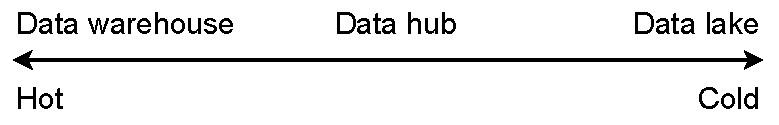
\includegraphics[width=0.5\textwidth]{img/_storage.pdf}
            \caption{Data storage technologies}
        \end{figure}
\end{description}


\section{Traditional vs insight-driven data systems}
\begin{tabular}{c | p{0.4\textwidth} | p{0.4\textwidth}}
    & \textbf{\makecell[c]{Traditional (data warehouse)}} & \textbf{\makecell[c]{Insight-driven (data lake)}} \\
    \hline
    \textbf{Sources} & Structured data & Structured, semi-structured and unstructured data \\
    \hline
    \textbf{Storage} & Limited ingestion and storage capability & Virtually unlimited ingestion and storage capability \\
    \hline
    \textbf{Schema} & Schema designed upfront & Schema not fixed \\
    \hline
    \textbf{Transformations} & \ac{etl} upfront & Transformations on query \\
    \hline
    \textbf{Analytics} & SQL, \ac{bi} tools, full-text search & Traditional methods, self-service \ac{bi}, big data, machine learning, \dots \\
    \hline
    \textbf{Price} & High storage cost & Low storage cost \\
    \textbf{Performance} & Fast queries & Scalability/speed/cost tradeoffs \\
    \hline
    \textbf{Quality} & High data quality & Depends on the use case \\
\end{tabular}


\section{Data architecture evolution}
\begin{description}
    \item[Traditional data warehouse] \marginnote{Traditional data warehouse} 
        (i.e. in-house data warehouse)
        \begin{itemize}
            \item Structured data with predefined schemas.
            \item High setup and maintenance cost. Not scalable.
            \item Relational high-quality data.
            \item Slow data ingestion.
        \end{itemize}

    \item[Modern cloud data warehouse] \marginnote{Modern cloud data warehouse} 
        \phantom{}
        \begin{itemize}
            \item Structured and semi-structured data.
            \item Low setup and maintenance cost. Scalable and easier disaster recovery.
            \item Relational high-quality data and mixed data.
            \item Fast data ingestion if supported.
        \end{itemize}

    \item[On-premise big data] \marginnote{On-premise big data} 
        (i.e. in-house data lake)
        \begin{itemize}
            \item Any type of data with schemas on read.
            \item High setup and maintenance cost.
            \item Fast data ingestion.
        \end{itemize}

    \item[Cloud data lake] \marginnote{Cloud data lake} 
        \phantom{}
        \begin{itemize}
            \item Any type of data with schemas on read.
            \item Low setup and maintenance cost. Scalable and easier disaster recovery.
            \item Fast data ingestion.
        \end{itemize}
\end{description}


\section{Components}

\subsection{Data ingestion} 
    \begin{descriptionlist}
        \item[Workload migration] \marginnote{Data ingestion}
            Inserting all the data from an existing source.
        \item[Incremental ingestion]
            Inserting changes since the last ingestion.
        \item[Streaming ingestion]   
            Continuously inserting data.
    \end{descriptionlist}

    \begin{description}
        \item[\Acl{cdc} (\Acs{cdc})] \marginnote{\Acl{cdc} (\Acs{cdc})}
            Mechanism to detect changes and insert the new data into the data lake (possibly in real-time).
    \end{description}

\subsection{Storage}
\begin{descriptionlist}
    \item[Raw] \marginnote{Raw storage}
        Immutable data useful for disaster recovery.
    \item[Optimized] \marginnote{Optimized storage}
        Optimized raw data for faster query.
    \item[Analytics] \marginnote{Analytics storage}
        Ready to use data.
\end{descriptionlist}

\begin{description}
    \item[Columnar storage] \phantom{}
        \begin{itemize}
            \item Homogenous data are stored contiguously.
            \item Speeds up methods that process entire columns (i.e. all the values of a feature).
            \item Insertion becomes slower.
        \end{itemize}

    \item[Data catalog]
        Methods to add descriptive metadata to a data lake.
        This is useful to prevent an unorganized data lake (data swamp).
\end{description}
        
\subsection{Processing and analytics} 
\begin{descriptionlist}
    \item[Interactive analytics] \marginnote{Processing and analytics}
        Interactive queries to large volumes of data.
        The results are stored back in the data lake.
    \item[Big data analytics]
        Data aggregations and transformations.
    \item[Real-time analytics]   
        Streaming analysis.
\end{descriptionlist}


\section{Architectures}

\subsection{Lambda lake} 
\begin{description}
    \item[Batch layer] \marginnote{Lambda lake}
        Receives and stores the data. Prepares the batch views for the serving layer.
    \item[Serving layer] 
        Indexes batch views for faster queries.
    \item[Speed layer] 
        Receives the data and prepares real-time views. The views are also stored in the serving layer.
\end{description}
\begin{figure}[ht]
    \centering
    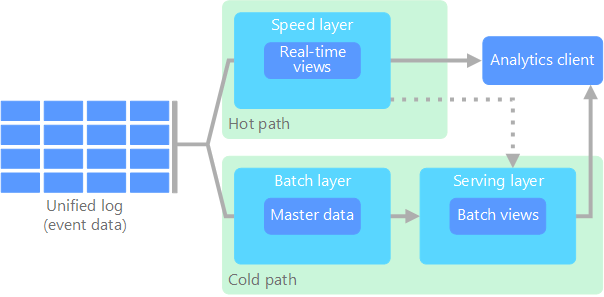
\includegraphics[width=0.5\textwidth]{img/lambda_lake.png}
    \caption{Lambda lake architecture}
\end{figure}

\subsection{Kappa lake} 
\marginnote{Kappa lake}
The data are stored in a long-term store.
Computations only happen in the speed layer (avoids lambda lake redundancy between batch layer and speed layer).
\begin{figure}[ht]
    \centering
    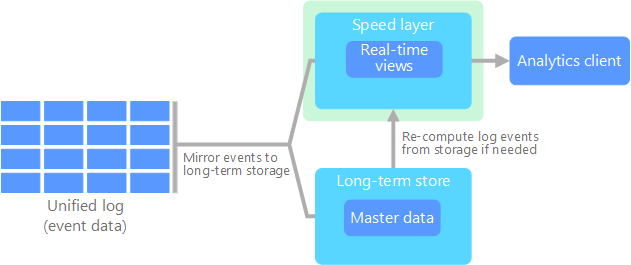
\includegraphics[width=0.5\textwidth]{img/kappa_lake.png}
    \caption{Kappa lake architecture}
\end{figure}

\subsection{Delta lake} 
\marginnote{Delta lake}
Framework that adds features on top of an existing data lake.
\begin{itemize}
    \item ACID transactions
    \item Scalable metadata handling
    \item Data versioning
    \item Unified batch and streaming
    \item Schema enforcement
\end{itemize}
\begin{figure}[ht]
    \centering
    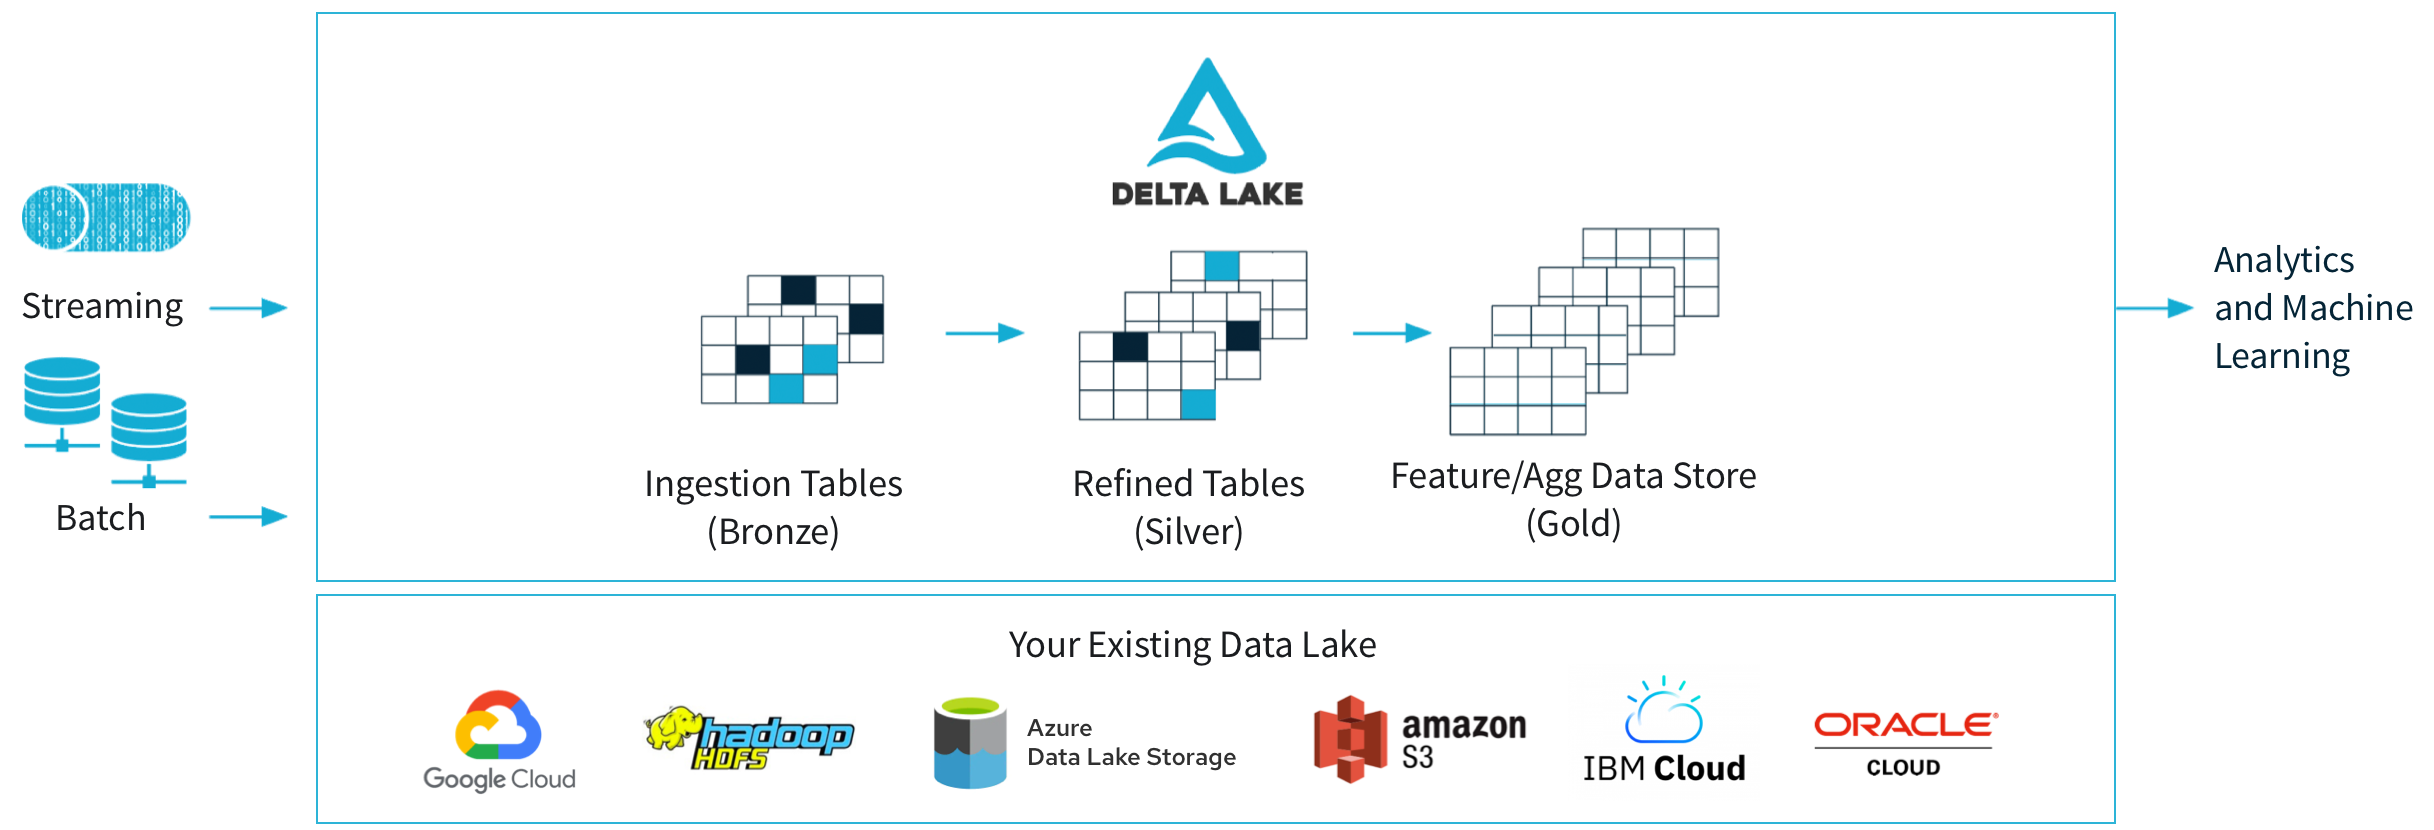
\includegraphics[width=0.7\textwidth]{img/delta_lake.png}
    \caption{Delta lake architecture}
\end{figure}


\section{Metadata}
\marginnote{Metadata}
Metadata is used to organize a data lake.
Useful metadata are:
\begin{descriptionlist}
    \item[Source] Origin of the data.
    \item[Schema] Structure of the data.
    \item[Format] File format or encoding.
    \item[Quality metrics] (e.g. percentage of missing values).
    \item[Lifecycle] Retention policies and archiving rules.
    \item[Ownership] 
    \item[Lineage] History of applied transformations or dependencies.
    \item[Access control] 
    \item[Classification] Sensitivity level of the data.
    \item[Usage information] Record of who accessed the data and how it is used.
\end{descriptionlist}